\documentclass[a4paper,12pt]{article}

\usepackage[a4paper]{geometry}

\usepackage[utf8]{inputenc}            % Use utf8 input encoding
%\usepackage[latin1]{inputenc}         % Use iso 8859-1 encoding
\usepackage[T1]{fontenc}               % T1 fonts (support for accents/diacritics)
\usepackage{lmodern}                   % font with proper T1 support and good glyph quality

\usepackage{listings}                  % for (code) listings
\lstset{language=Java}
\usepackage{amsmath}                   % AMS math typesetting
\usepackage{titlesec}

\usepackage{hyperref}                  % better references for PDF

\usepackage{graphicx}               % for graphics
\usepackage{float}
\usepackage{caption}

\usepackage{pdfpages}

\titleformat{\section}{\LARGE\bfseries}% hide redundant number
            {}{0pt}{}
            
\graphicspath{{pictures/assignment4/}}

\begin{document}

\begin{center}
	\rule{\textwidth}{0.1pt}\\[1cm]
	
	\Large Softwarepraktikum SS 2019\\\bf Assignment 4
\end{center}


\begin{center}

	\rule{\textwidth}{0.1pt}\\[0.5cm]

	{\Large Group - 6\\[5mm]}

	\begin{tabular}{lll}

		Roman Vuskov & 376809 & roman.vuskov@rwth-aachen.de \\

		Songran Shi & 357791 & songran.shi@rwth-aachen.de \\

		Marlene Damm & 379945 & marlene.damm@rwth-aachen.de \\
		
		Marvin Gazibarić & 378154 & marvin.gazibaric@rwth-aachen.de \\

	\end{tabular}\\[0.5cm]

	\rule{\textwidth}{0.1pt}\\[1cm]

\end{center}

% Uncomment next two lines for table of contents
\newpage
%\tableofcontents

\section{Task 1}

In assignment 3, we already implemented a beam search algorithm. The moves are evaluated and the best $k$ moves are sorted into a list we call the search beam while all other moves are discarded. $k$ is therefore the \emph{beam width}. \emph{Move sorting}, in comparison, is thus equivalent to setting $k=\infty$, i.e. without discarding any moves.
\\ \\
Implementation-wise we could have used our beam search with beam width set to a very high value. But this would have resulted in a heavy performance penalty since the $\mathcal O(n\cdot k)$\footnote{$n$ is the number of moves in a given game state.}, 
algorithm we use to sort our beam would degenerate to complexity $\mathcal O(n^2)$. Instead we implemented a dedicated move sorting method \texttt{getOrderedMoves()} that uses a heavily optimized $\mathcal O(n\log n)$ sorting mechanism from the Java standard library.
\\ \\
Additionally, we also allowed the option of not sorting moves at all for completeness' sake, although this is highly discouraged as it renders alpha-beta pruning and the upcoming aspiration windows essentially useless.

\newpage

\section{Task 3}
For this exercise, we implemented two new classes, \texttt{IterationHeuristic} and \texttt{PancakeWatchdog} to help our AI realize iterative deepening.
\\ \\
\texttt{IterationHeuristic} is used in between iterations of depth searches to estimate whether there is sufficient time for one more step in depth. Every iteration the method \texttt{doIteration()} is called, returning \texttt{true} when iterative deepening should be proceeded.
\\ \\
Currently the implementation is very basic. It aborts, i.e. returns \texttt{false}, if a certain time threshold is exceeded. That threshold is just $T\cdot h$, where $T$ is the time limit for that particular move and $h$ a hardcoded value, set to $h=0.2$. We assume that search time scales linearly with number of nodes. Given that our beam width $n$ is set to 5 per default, that value seems reasonable. This procedure works astonishingly well, with regard to its simplicity, but we still intend to implement more refined game-stage dependent time budget management in the future.
\\ \\
\texttt{PancakeWatchdog} is a safeguard against timeout disqualifications in case our iteration heuristic underestimated the time needed to complete the next iteration of depth search and gave it green light despite time shortage. The time check method \texttt{isPancake()} gets called frequently during the actual depth search, both in \texttt{evaluateNode()} and \texttt{getBeamMoves()}, to catch any impending timeout before it occurs with a safety margin currently set to $100 ms$.

\begin{figure}[H]
    \centering
    
\includegraphics[height=5cm]{pictures/assignment4/burned_pancake.jpg}
    \caption*{Nobody likes burnt pancakes, so be sure to turn off the heat 100 ms early!}
    \label{fig:burned_pancake}
\end{figure}

To sum up, iterative deepening is realized by a \texttt{while}-loop in our AI class that calls \texttt{BRSNode} repeatedly with increasing depth limit so long as \texttt{IterationHeuristic} considers time budget abundant, and any false estimatates are caught by the \texttt{PancakeWatchdog}. The best move is updated with the best move of each search iteration. In case a search is terminated prematurely, the best move of that iteration remains \texttt{null} and the result from previous iterations are used instead.

\begin{figure}[H]
    \centering
    
\includegraphics[height=5cm]{pictures/assignment4/pancakes_and_bacon.jpg}
    {\caption*{Bacon and pancakes, a timeless duo}}
    \label{fig:pancakes_and_bacon}
\end{figure}

\section{Task 2}
Below we provide graphs showing the time efficiency of constant depth searches with and without move sorting and beam search. It is apparent that time per move is highly correlated with number of states evaluated. As expected, sorting moves according to heuristic values results in a moderate speedup (3-10x) compared with no-move-ordering searches due to more pruning opportunities. This, conversely, gives us confidence that our board state rating heuristics are at least self-consistent, i.e. board states with high heuristic values tend to produce child nodes also with high heuristic values. \\ \\
Of course, beam search produces an even greater speedup (up to 100x) compared with no-move-ordering searches. More importantly, with beam search time per move remains nearly constant throughout the game, while without beam search time per move jumps wildly depending on how many moves are available in a particular board configuration (generally starts out low in early game and reaches local maximum in mid- to late-game, then explodes in ``override phase''). Practically speaking, we would have to continue using beam search or implement far faster heuristics in order to not exceed the standard 1 second time limit.

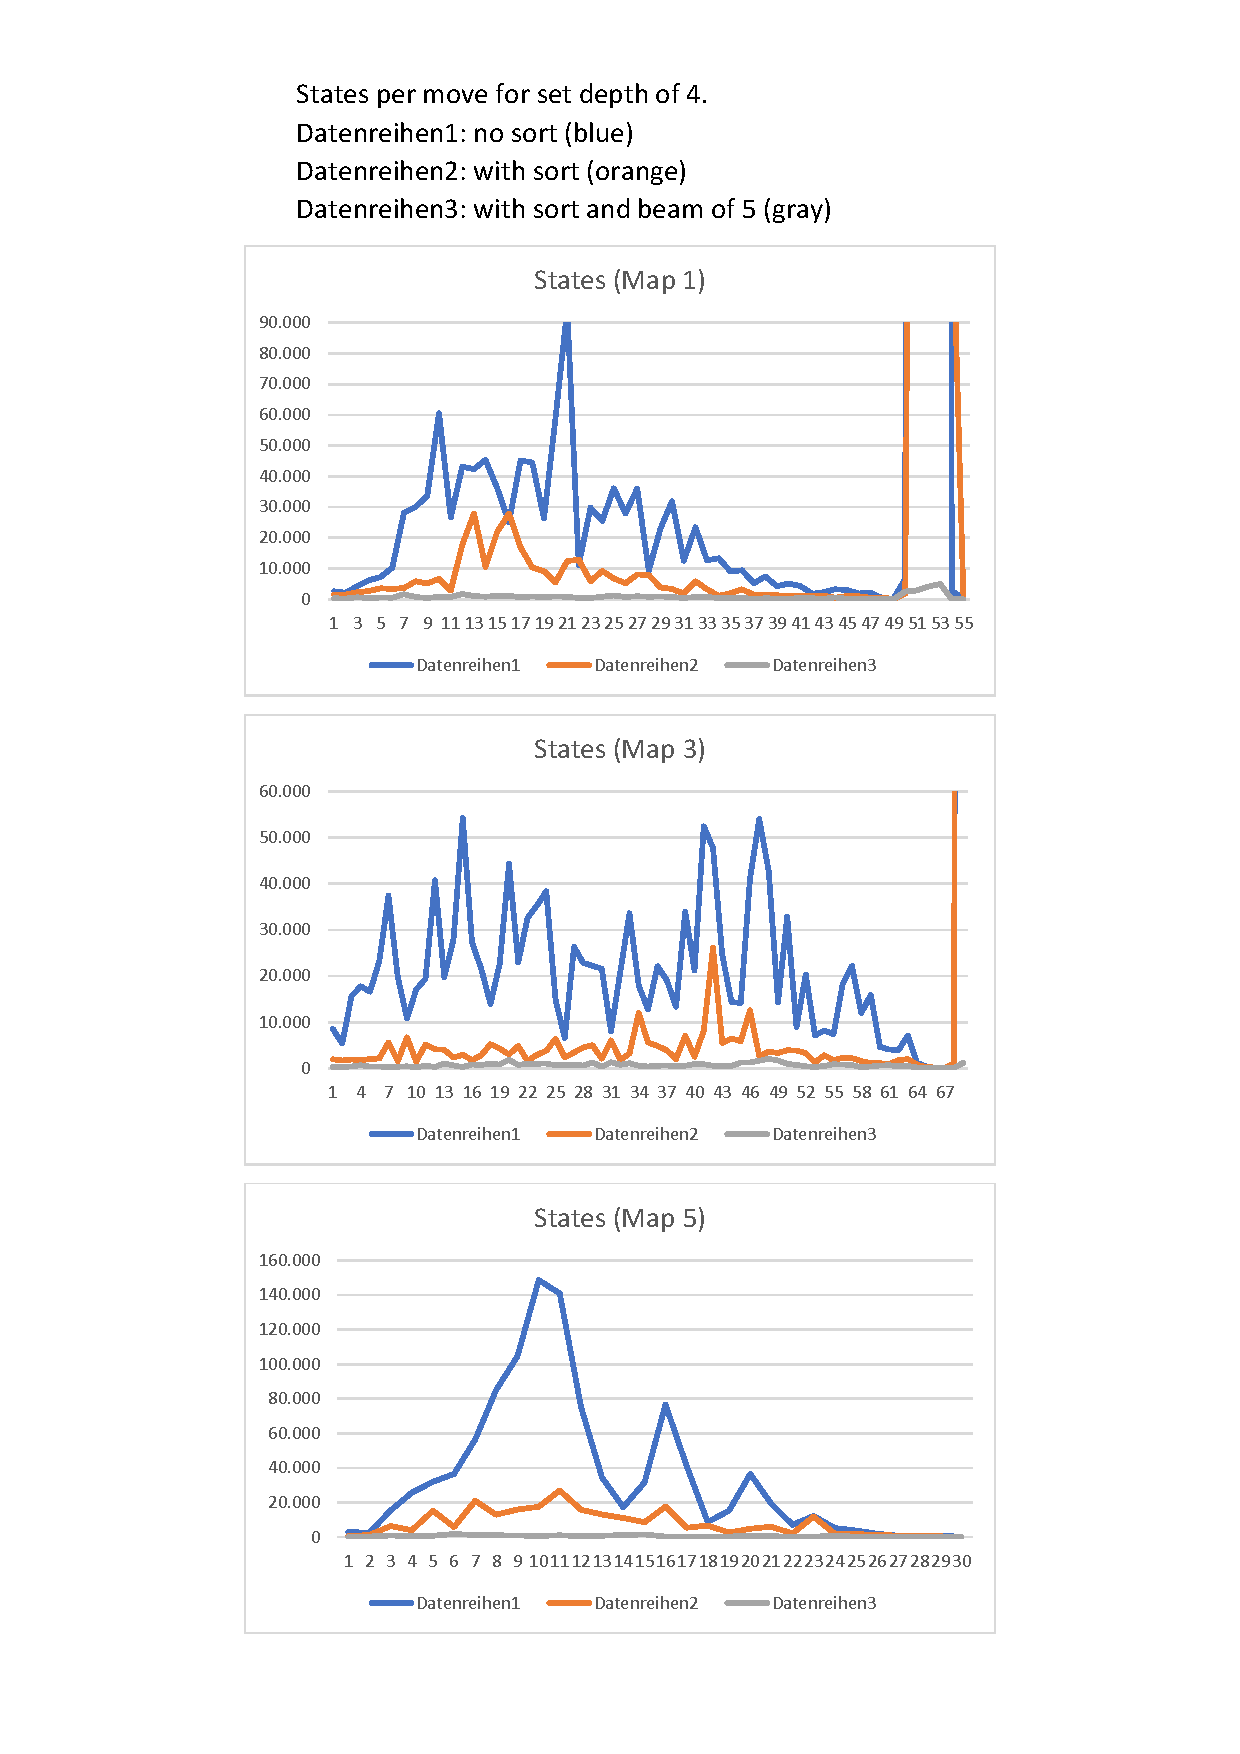
\includepdf[pages={1,2,3,4}]{exelPdf/statesDepth.pdf}
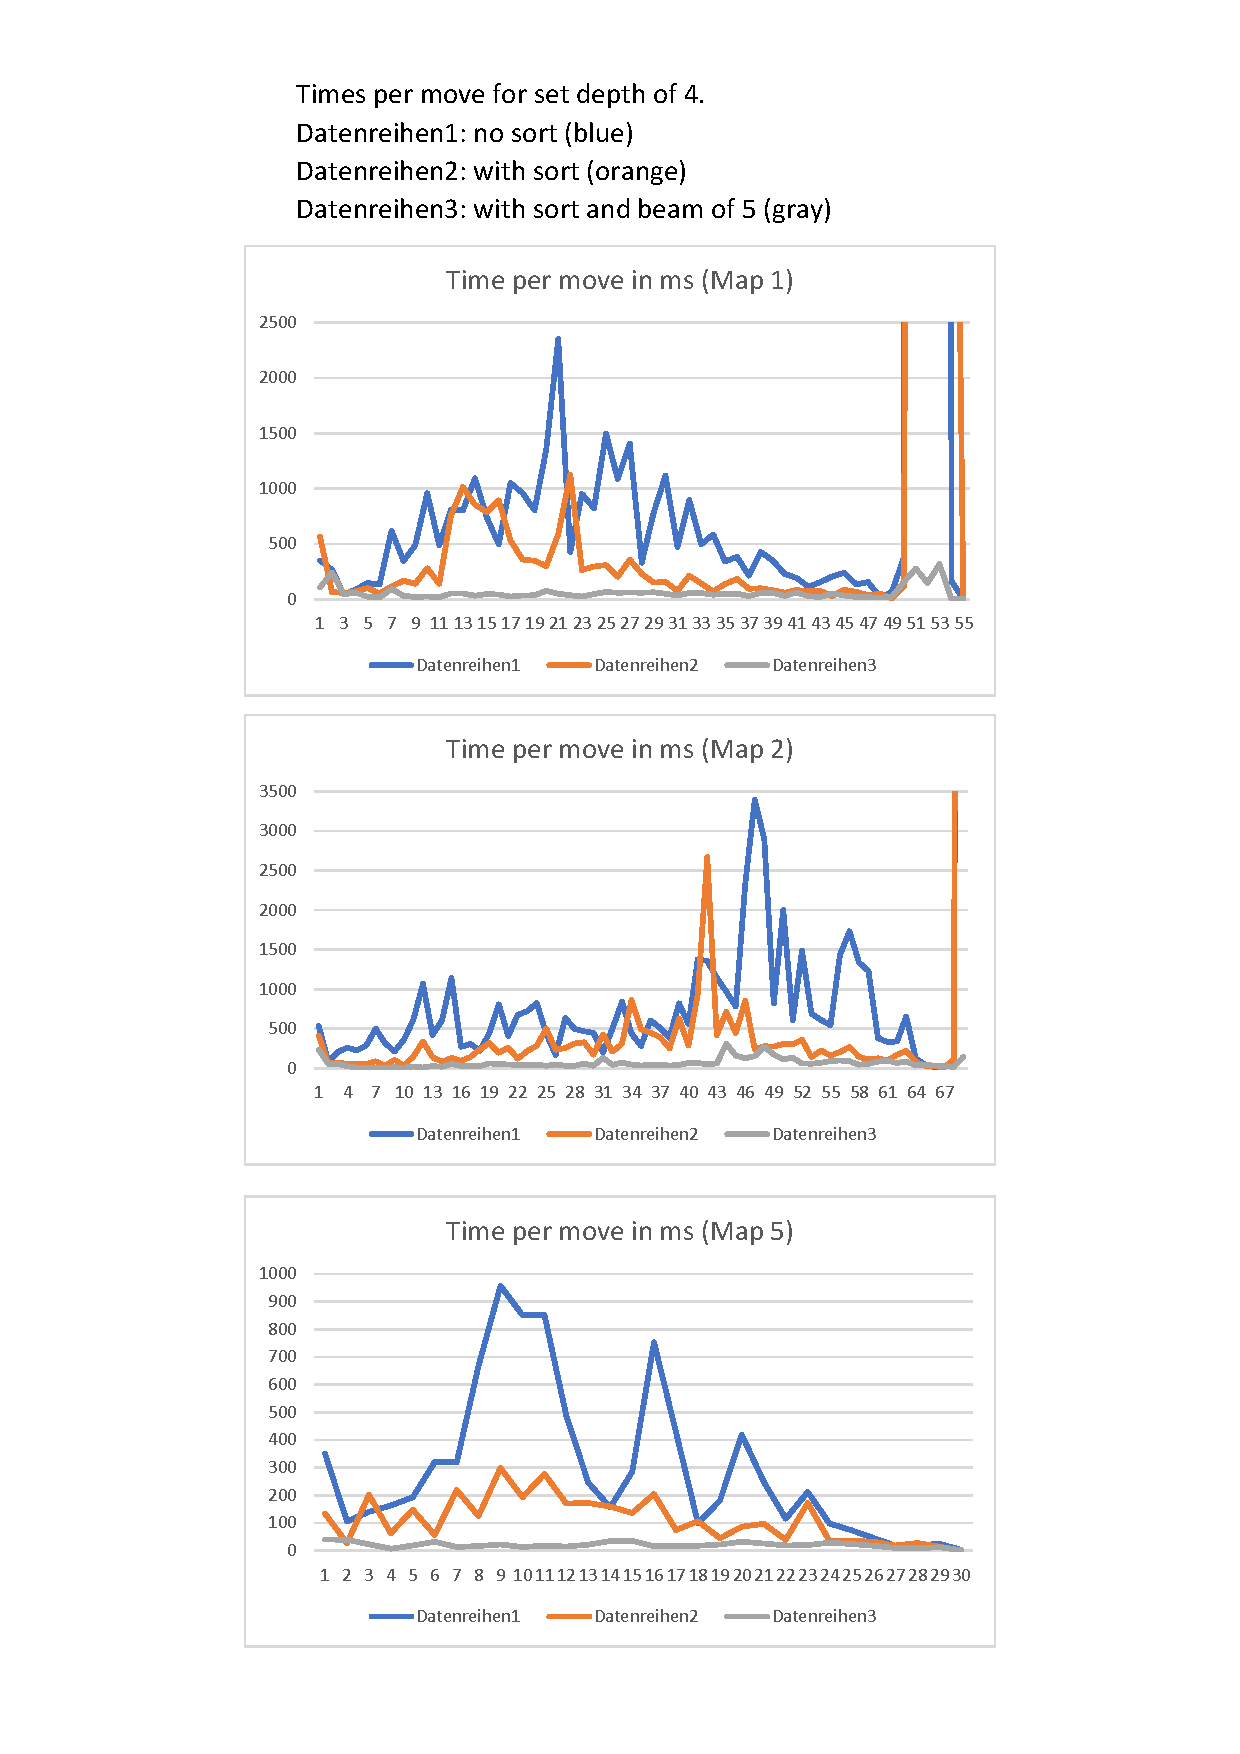
\includepdf[pages={1,2,3,4}]{exelPdf/timesPerMove.pdf}
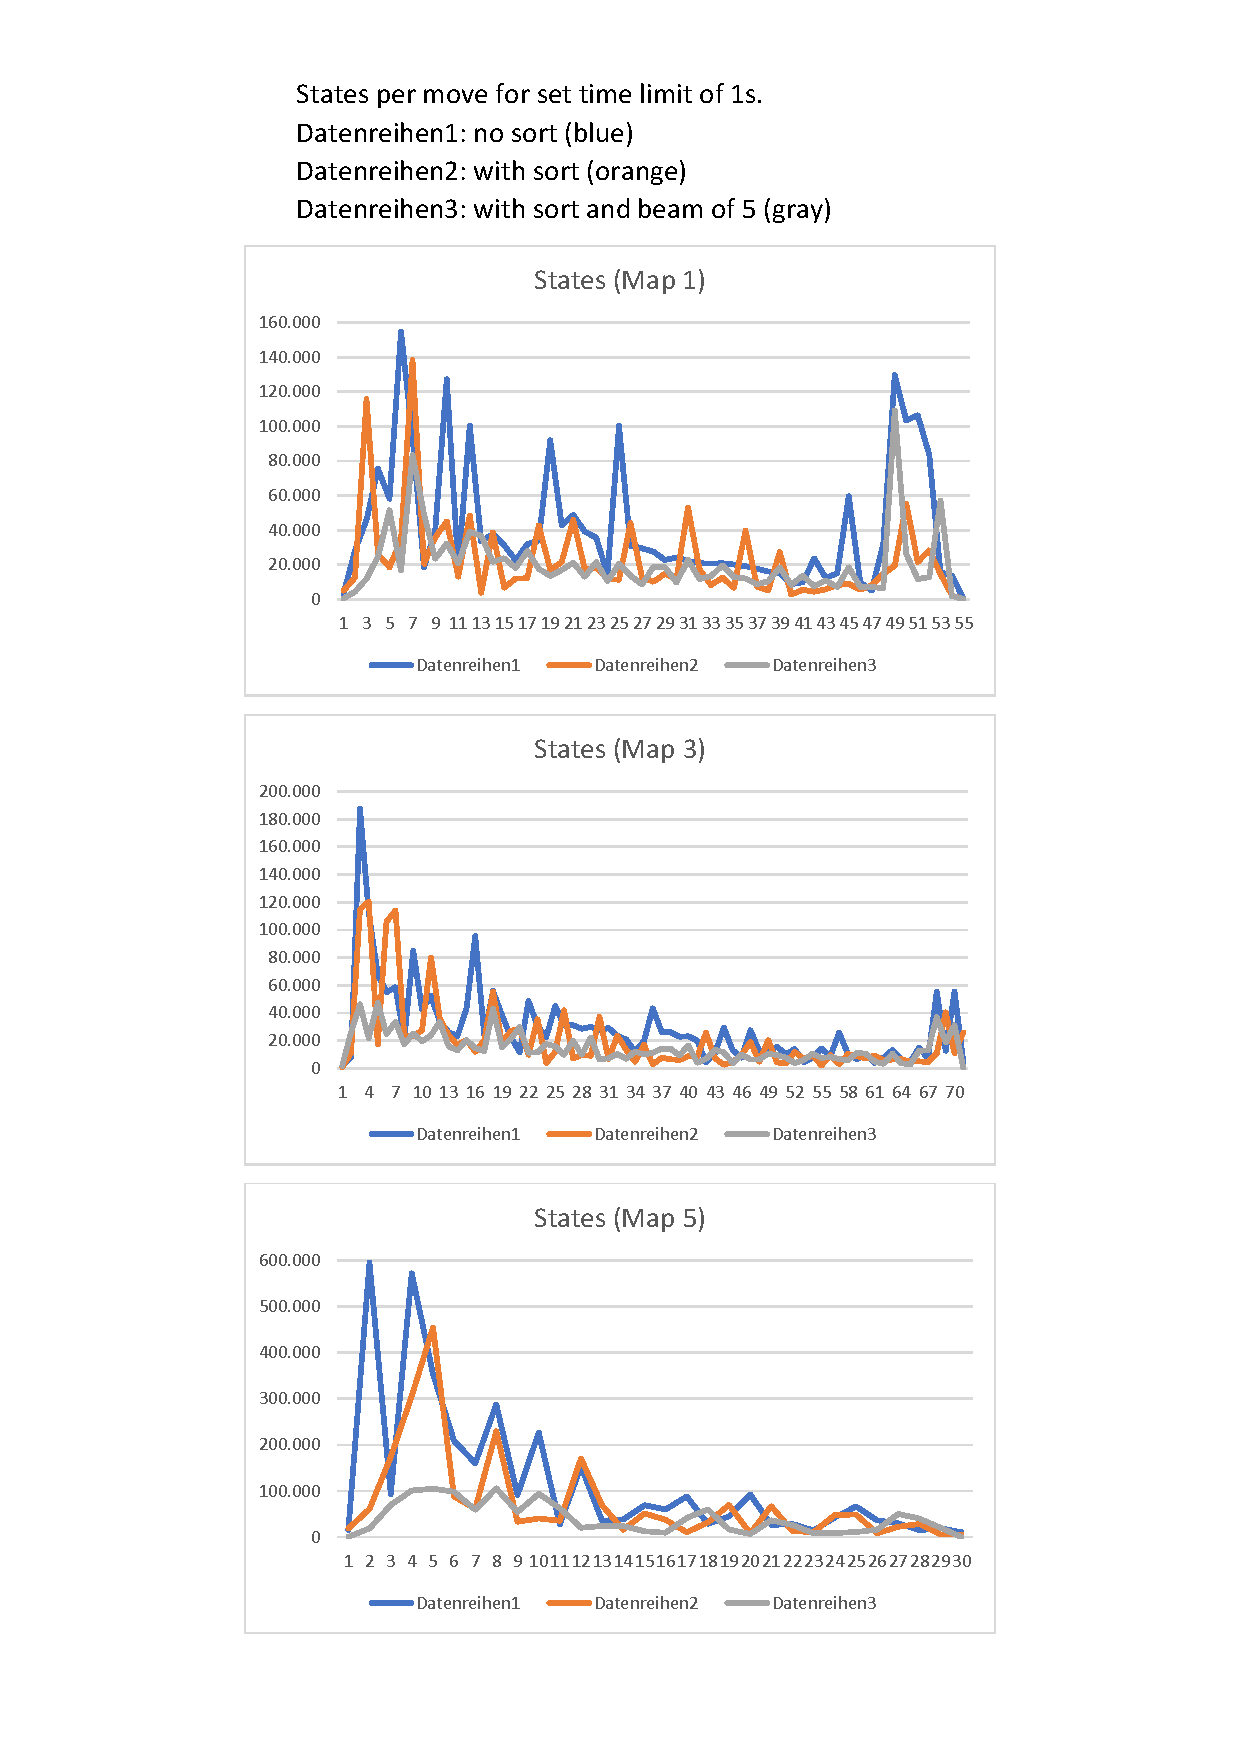
\includepdf[pages={1,2,3,4}]{exelPdf/statesTime.pdf}
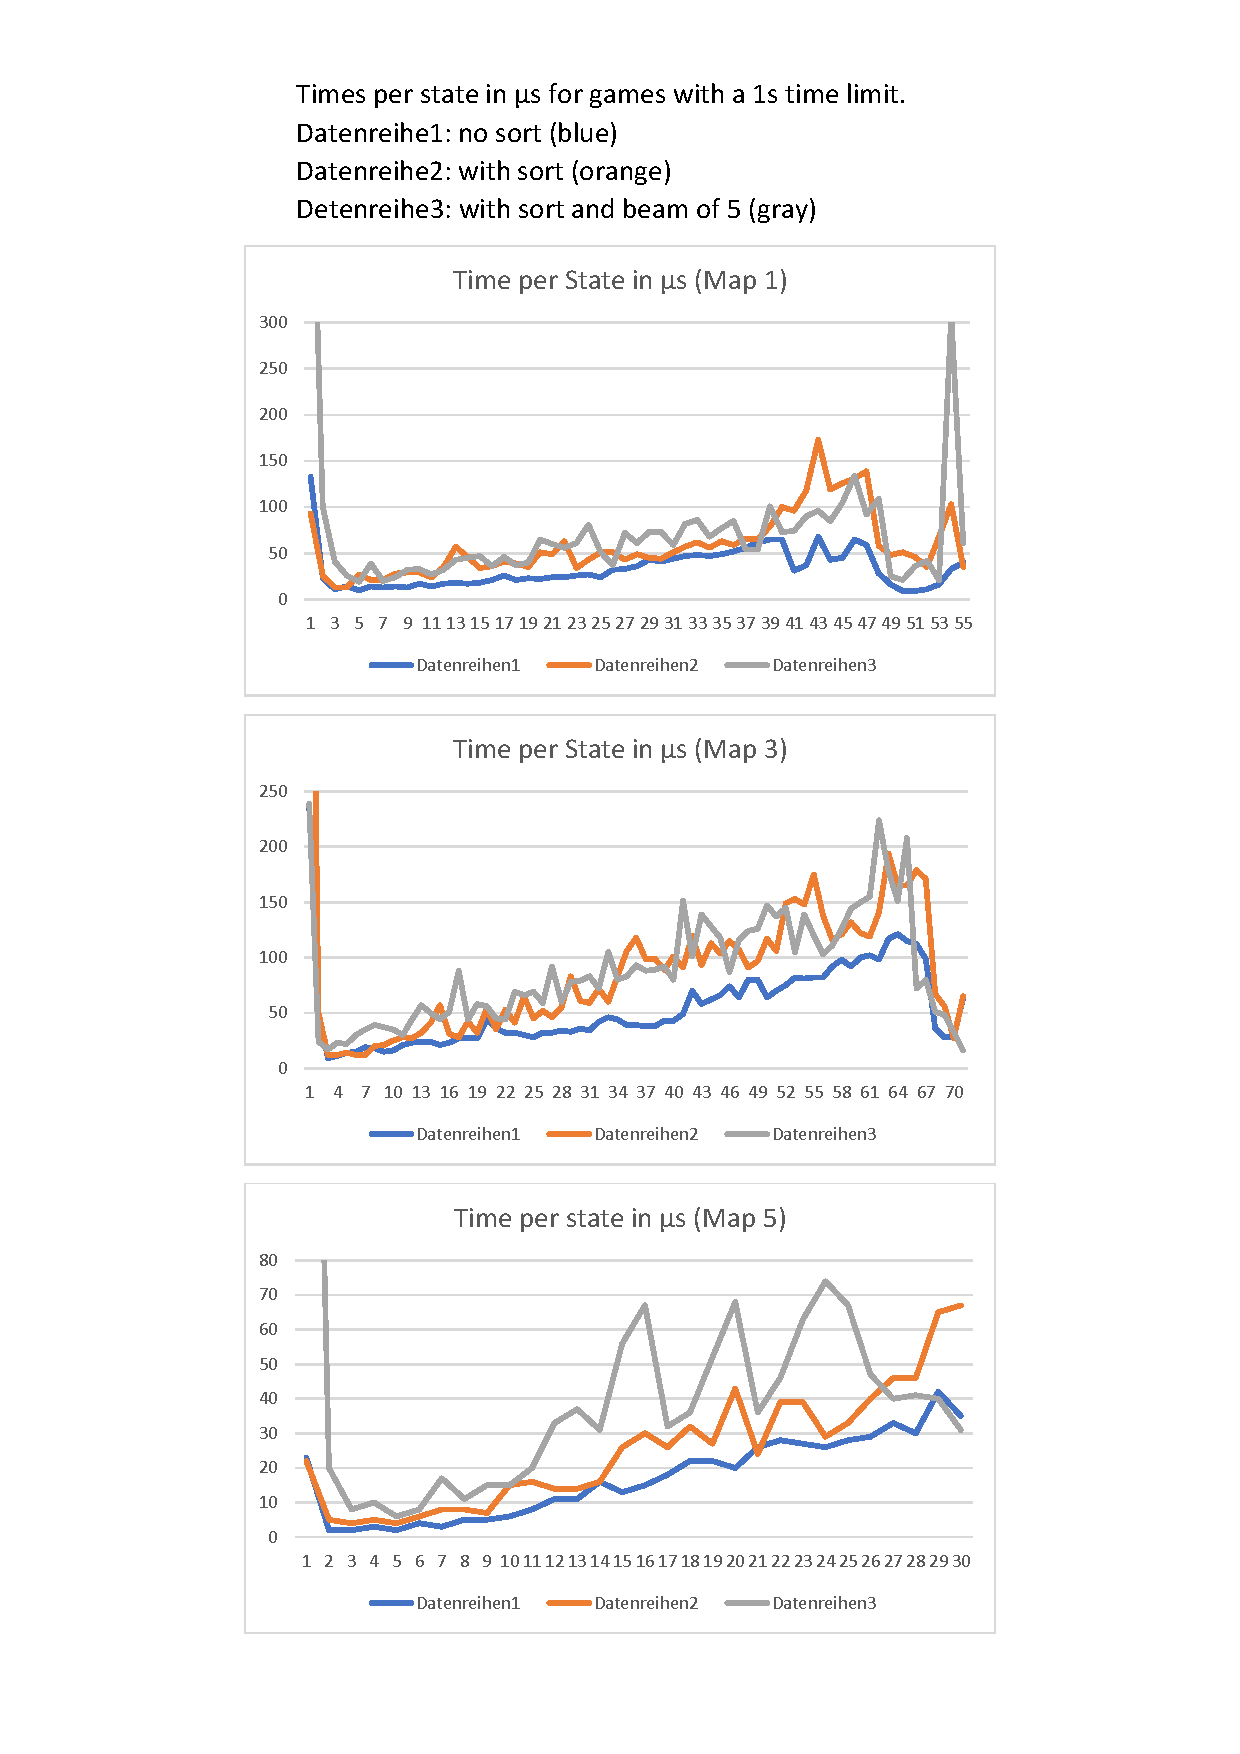
\includepdf[pages={1,2,3,4}]{exelPdf/timesPerState.pdf}
\end{document}

